\newcommand{\ubit}[1]{$u_{#1}$}
\newcommand{\fbit}[1]{\color{gray}$u_{#1}$}
\newcommand{\ucw}[1]{$x_{#1}$}
\newcommand{\fcw}[1]{\color{gray}$x_{#1}$}
\newcommand{\ub}[1]{$#1$}
\newcommand{\fb}[1]{\color{gray}$#1$}

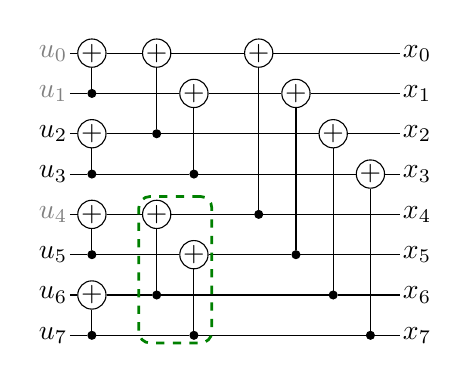
\begin{tikzpicture}

\usetikzlibrary{shapes,positioning,arrows,decorations.markings,fit}

\definecolor{varnode_fill}{RGB}{0,0,0}
\definecolor{chknode_fill}{RGB}{255,255,255}

\tikzset{
  chknode/.style={draw,fill=chknode_fill,circle,minimum size=0.3cm, inner sep=0},
  varnode/.style={draw,fill=varnode_fill,circle,minimum size=0.1cm, inner sep=0},
  channel/.style={draw,fill=white,rectangle},
  sep/.style={rectangle,minimum width=0.25cm, inner sep=0},
  empty/.style={rectangle, inner sep=0},
  bit/.style={circle, inner sep = 0}
}

\tikzset{green dotted/.style={draw=green!50!black, line width=1pt,
    dash pattern=on 3pt off 3pt,
    inner sep=0.4mm, rectangle, rounded corners}};

\matrix[row sep=1mm, column sep=1mm] {
  \node[bit] (n0s0) {\fb{u_0}}; & \node[chknode] (n0s1) {$+$}; & \node[sep] (s10) {}; & \node[chknode] (n0s2) {$+$}; & \node[empty] {};              & \node[sep] (s20) {}; & \node[chknode] (n0s3) {$+$}; & \node[empty] {}; & \node[empty] {}; & \node[empty] {}; && \node[bit] (xn0s4) {\ub{x_0}};\\
  \node[bit] (n1s0) {\fb{u_1}}; & \node[varnode] (n1s1) {};    & \node[sep] (s11) {}; &                              & \node[chknode] (n1s2) {$+$};  & \node[sep] (s21) {}; & \node[empty] {};             & \node[chknode] (n1s3) {$+$}; & \node[empty] {}; & \node[empty] {}; && \node[bit] (xn1s4) {\ub{x_1}};\\
  \node[bit] (n2s0) {\ub{u_2}}; & \node[chknode] (n2s1) {$+$}; & \node[sep] (s12) {}; & \node[varnode] (n2s2) {};    & \node[empty] {};              & \node[sep] (s22) {}; & \node[empty] {};             & \node[empty] {}; & \node[chknode] (n2s3) {$+$}; & \node[empty] {}; && \node[bit] (xn2s4) {\ub{x_2}};\\

  \node[bit] (n3s0) {\ub{u_3}}; & \node[varnode] (n3s1) {};    & \node[sep] (s13) {}; & \node[empty] {};             & \node[varnode] (n3s2) {};     & \node[sep] (s23) {}; & \node[empty] {};             & \node[empty] {}; & \node[empty] {}; & \node[chknode] (n3s3) {$+$}; && \node[bit] (xn3s4) {\ub{x_3}};\\

  \node[bit] (n4s0) {\fb{u_4}}; & \node[chknode] (n4s1) {$+$}; & \node[sep] (s14) {}; & \node[chknode] (n4s2) {$+$}; & \node[empty] {};              & \node[sep] (s24) {}; & \node[varnode] (n4s3) {};    & \node[empty] {}; & \node[empty] {}; & \node[empty] {}; && \node[bit] (xn4s4) {\ub{x_4}};\\
  \node[bit] (n5s0) {\ub{u_5}}; & \node[varnode] (n5s1) {};    & \node[sep] (s15) {}; &                              & \node[chknode] (n5s2) {$+$};  & \node[sep] (s25) {}; & \node[empty] {};             & \node[varnode] (n5s3) {}; & \node[empty] {}; &  \node[empty] {}; && \node[bit] (xn5s4) {\ub{x_5}};\\
  \node[bit] (n6s0) {\ub{u_6}}; & \node[chknode] (n6s1) {$+$}; & \node[sep] (s16) {}; & \node[varnode] (n6s2) {};    & \node[empty] {};              & \node[sep] (s26) {}; & \node[empty] {};             & \node[empty] {}; & \node[varnode] (n6s3) {}; &  \node[empty] {}; && \node[bit] (xn6s4) {\ub{x_6}};\\
  
  \node[bit] (n7s0) {\ub{u_7}}; & \node[varnode] (n7s1) {};    & \node[sep] (s17) {}; &                              & \node[varnode] (n7s2) {};  & \node[sep] (s27) {}; & \node[empty] {};             & \node[empty] {}; & \node[empty] {}; &  \node[varnode] (n7s3) {}; && \node[bit] (xn7s4) {\ub{x_7}};\\
};
\path[-] (n0s0) edge (n0s1) (n0s1) edge (n0s2) (n0s2) edge (n0s3) (n0s3) edge (xn0s4);
\path[-] (n1s0) edge (n1s1) (n1s1) edge (n1s2) (n1s2) edge (n1s3) (n1s3) edge (xn1s4);
\path[-] (n2s0) edge (n2s1) (n2s1) edge (n2s2) (n2s2) edge (n2s3) (n2s3) edge (xn2s4);
\path[-] (n3s0) edge (n3s1) (n3s1) edge (n3s2) (n3s2) edge (n3s3) (n3s3) edge (xn3s4);
\path[-] (n4s0) edge (n4s1) (n4s1) edge (n4s2) (n4s2) edge (n4s3) (n4s3) edge (xn4s4);
\path[-] (n5s0) edge (n5s1) (n5s1) edge (n5s2) (n5s2) edge (n5s3) (n5s3) edge (xn5s4);
\path[-] (n6s0) edge (n6s1) (n6s1) edge (n6s2) (n6s2) edge (n6s3) (n6s3) edge (xn6s4);
\path[-] (n7s0) edge (n7s1) (n7s1) edge (n7s2) (n7s2) edge (n7s3) (n7s3) edge (xn7s4);

\path[-] (n0s1) edge (n1s1);
\path[-] (n2s1) edge (n3s1);
\path[-] (n4s1) edge (n5s1);
\path[-] (n6s1) edge (n7s1);

\path[-] (n0s2) edge (n2s2);
\path[-] (n1s2) edge (n3s2);
\path[-] (n4s2) edge (n6s2);
\path[-] (n5s2) edge (n7s2);

\path[-] (n0s3) edge (n4s3);
\path[-] (n1s3) edge (n5s3);
\path[-] (n2s3) edge (n6s3);
\path[-] (n3s3) edge (n7s3);

\node (g_n1s2) [green dotted, fit = (n4s2) (n5s2) (n6s2) (n7s2)] {};

\end{tikzpicture}
